\documentclass[11pt,a4paper]{article}

\usepackage[utf8]{inputenc}
\usepackage[german]{babel}
\usepackage[T1]{fontenc}
\usepackage{helvet}
\renewcommand{\familydefault}{\sfdefault}
\usepackage[left=2cm,right=2cm,top=2cm,bottom=2cm]{geometry}
\usepackage{csquotes}
\MakeOuterQuote{"}
\usepackage{graphicx}
\graphicspath{ {./src/} }

\renewcommand{\refname}{Referenzen}
\renewcommand{\figurename}{Abbildung}
\renewcommand{\tablename}{Tabelle}

\title{Medical Assistent}
\author{Adrian Locher, Jason Benz}
\date{\today}


\begin{document}
\pagenumbering{gobble}
\maketitle
\tableofcontents
\newpage

\pagenumbering{arabic}

\section{Einleitung}
    \subsection{Motivation}
        \paragraph{}
            Die Frage, ob ein Arzt besucht werden soll, ist häufig ein Dilemma.
            Einerseits, will man nicht diejenige Person sein, welche bei unbedenklichen Symptomen
            überreagiert, andererseits könnten sich die Symptome ja verschlimmern und vielleicht
            hätte der Arztbesuch das Problem frühzeitig beheben können. Ausserdem ist man schliesslich
            versichert.
            
        \paragraph{}
            Eine ganz andere Beudeutung hat dieses Dilemma ausserdem seit dem Anfang
            der Covid-19 Situation. Ärzte und anderes Gesundheitspersonal, gelten als besonders
            stark ausgelastet. Auf der Kehrseite hingegen, sollte man bei Covid-19-artigen Symptomen
            auch nicht zögern und sich testen lassen. Welche Symptome nun genau als "Covid-Symptome"
            gelten und welche nicht, ist teilweise sehr unübersichtlich, was die lage auch nicht
            einfacher werden lässt.

        \paragraph{}
            Das Ziel unseres Projekts, soll sein eine lösung zu entwickeln, mit der unnötige Arztbesuche
            generell, aber besonders in Situationen wie jetzt vermieden werden können.
            Das Ziel ist nicht, dass einfach grundsätzlich weniger Menschen Arztbesuche machen, sondern
            vielmehr, in Grenzfällen bei der Entscheidung zu helfen.
        
        \paragraph{}
            Um dabei auch wirklich das Gesundheitspersonal maximal zu entlasten, besteht unser
            Lösungsansatz nicht etwa aus einer Hotline. Ziel ist es ein AI gestützes System zu entwickeln,
            welches ganz ohne Menschliche Interaktion auskommt.


\newpage

\section{Java Client}
	Der Java Client ist in die folgenden drei Bereiche aufgeteilt, welche in den nachfolgenden Unterkapitel genauer beschrieben werden:
	\begin{enumerate}
		\item Command Line Interface
		\item Dialogflow Connector
		\item Medical Assistant
	\end{enumerate}
	
	\subsection{Command Line Interface}
		Beim Start des Medical Assistants im Java Client wird der User auf folgende Möglichkeiten hingewiesen:
		\begin{itemize}
			\item Input mit dem medizinischen Problem angeben
			\item "q" um den Assistenten wieder zu beenden
			\item "v" um den persönlichen medizinischen Bericht anzuschauen
		\end{itemize}
		%
		Die logische Abfolge des Benutzerinputs, bzw. die Interaktion mit dem Dialogflow Chatbot ist analog zum beschriebenen Ablauf in Abildung \ref{fig:backEndFlowChart}. Nach jeder Antwort des Chatbots können die Optionen "q" und "v" aufgerufen werden.
	
	\subsection{Dialogflow Connector}
		Beim Projekttyp handelt es sich um ein Maven-Projekt. Für die Interaktion mit Dialogflow wurde das Artefakt "google-cloud-dialogflow" verwendet.
		
		\paragraph{}
		Die Einbindung, sowie die Basisimplementierung (Dialogflow Kommunikation) war bereits Bestandteil einer Übungsstunde. Deshalb wird dies als Vorwissen angeschaut und in diesem Report nicht weiter thematisiert. Projektspezifische Anwendungsfälle werden in den entsprechenden Kapiteln beschrieben.
	
	\subsection{Medical Assistant Implementation}
		\subsubsection{Report}
			Neben der Interaktion mit dem Dialogflow Chatbot ist das Hauptziel des Java Clients, dem Benutzer einen medizinischen Bericht zur Verfügung zu stellen. Wenn dieser mit dem CLI Kommando "v" abgerufen wird, ist dieser zu Beginn leer:
			\begin{figure}[h!]
				\begin{center}
            		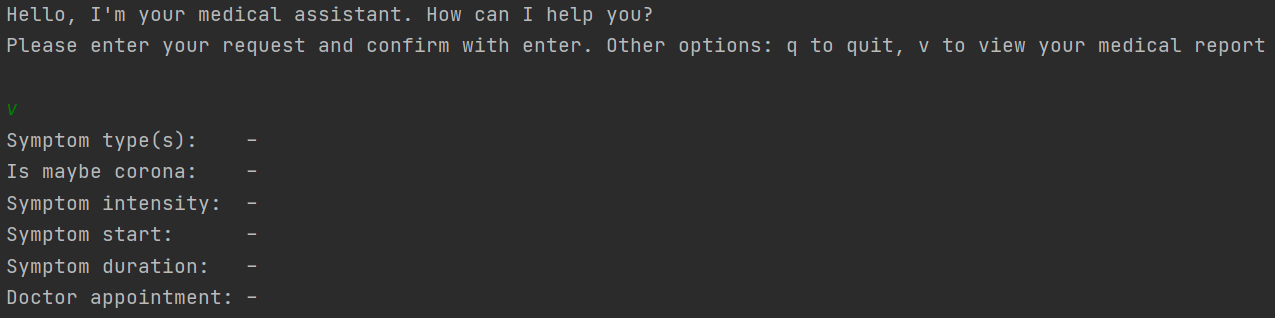
\includegraphics[width=0.85\linewidth]{JavaClient-EmptyReport.png}
		            \caption{Leerer medizinischer Report}
		            \label{fig:javaClient_emptyReport}
				\end{center}
	        \end{figure}
	        
	        Fortlaufend - basierend auf den User-Inputs, sowie den Chatbot Antworten - wird der Report ergänzt (siehe: \ref{sssec:intent_handling}). Am Ende kann der ausgefüllte Bericht zum Beispiel folgendermassen aussehen:
			\begin{figure}[h!]
				\begin{center}
            		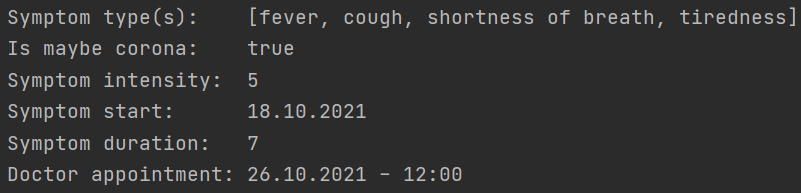
\includegraphics[width=0.65\linewidth]{JavaClient-CompletedReport.png}
		            \caption{Komplett ausgefüllter Beispiel-Report}
		            \label{fig:javaClient_completedReport}
				\end{center}
	        \end{figure}
		
		\subsubsection{Intent Handling} \label{sssec:intent_handling}			
		Die für den Java Client relevanten Intents sind \emph{"check\_symptoms"}, sowie der Folge-Intent \emph{"check\_symptoms - yes - time"}. Via Switch-Case Statement werden Intent-spezifische Aktionen durgeführt, welche schlussendlich den medizinischen Bericht aktualisieren. \\\\
		
		\underline{\emph{Intent "check\_symptoms"}} \\
		\begin{enumerate}
			\item Via Dialogflow Backend wird dynamisch anhand der Symptome ermittelt, ob der Benutzer eventuell Corona hat. Diese Information wird über den Payload an den Java Client übermittelt. Das Query-Result im Java Code enthält die Methode \emph{"getWebhookPayload()"}, welche den Zugriff auf den Payload als Struct ermöglicht. Auf dieser Datenbasis wird der Report entsprechend um das Attribut \emph{"hasMaybeCorona"} ergänzt.
			\begin{figure}[h!]
				\begin{center}
            		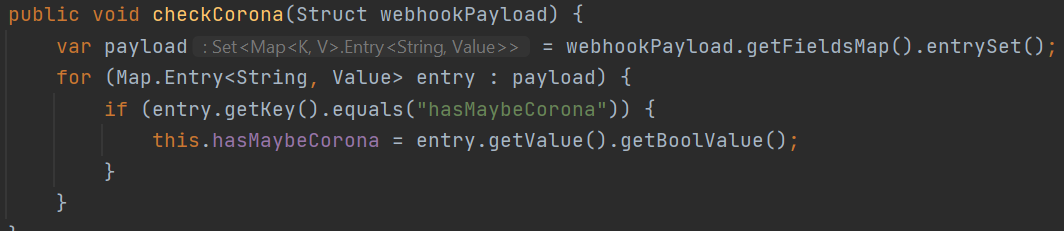
\includegraphics[width=0.8\linewidth]{JavaClient-CoronaCheck.png}
					\caption{Corona Payload zum Report hinzufügen}
					\label{fig:javaClient_coronaCheck}
				\end{center}
			\end{figure}
			
			\item Im nächsten Schritt werden alle aktualisierten Parameter auf dem Report im Java Client hinterlegt. Nachfolgend ist ein Ausschnitt der Aktualisierung des ersten Parameters zu sehen. Alle anderen Parameter werden im Swicht-Case Statement analog zu diesem Beispiel aktualisiert.
			\begin{figure}[h!]
				\begin{center}
            		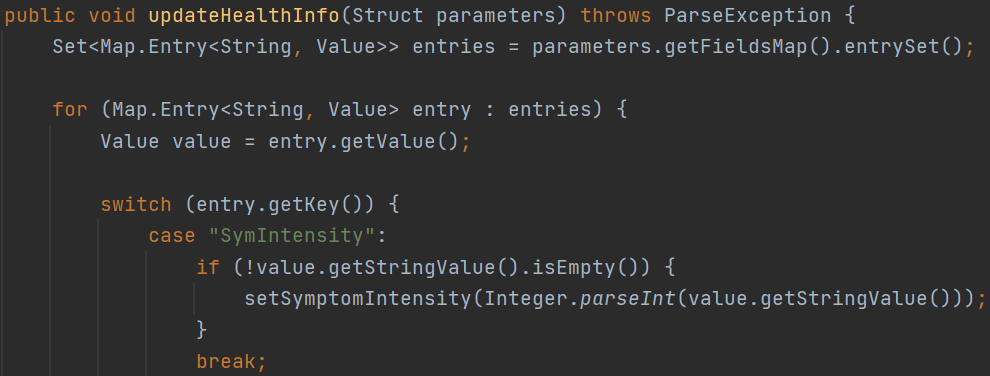
\includegraphics[width=0.8\linewidth]{JavaClient-ParameterHandling.png}
					\caption{Ausschnitt der Report Aktualisierung}
					\label{fig:javaClient_parameterHandling}
				\end{center}
			\end{figure}
		\end{enumerate}
		
		\underline{\emph{Intent "check\_symptoms - yes - time"}} \\
		\begin{enumerate}
			\item In diesem Intent wird noch der Arzttermin auf dem Report aktualisiert.
			\begin{figure}[h!]
				\begin{center}
            		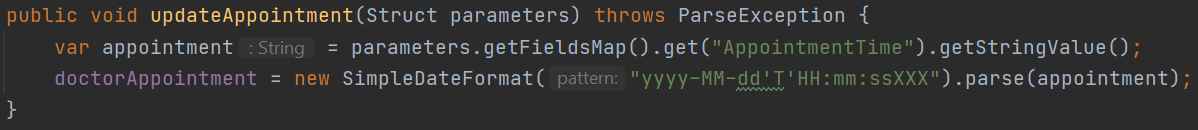
\includegraphics[width=1.0\linewidth]{JavaClient-UpdateAppointment.png}
					\caption{Arzttermin auf dem Report hinzufügen}
					\label{fig:javaClient_updateAppointment}
				\end{center}
			\end{figure}
		\end{enumerate}
	        
\newpage

\section{Backend}
    \subsection{Übersicht}
        \paragraph{}
        In Abbildung \ref{fig:backEndFlowChart} ist der logische Ablauf, des Dialogflows zu sehen, welcher das
        Backend unseres Chatbots bildet.
        \begin{figure}[h!]
            \begin{center}
                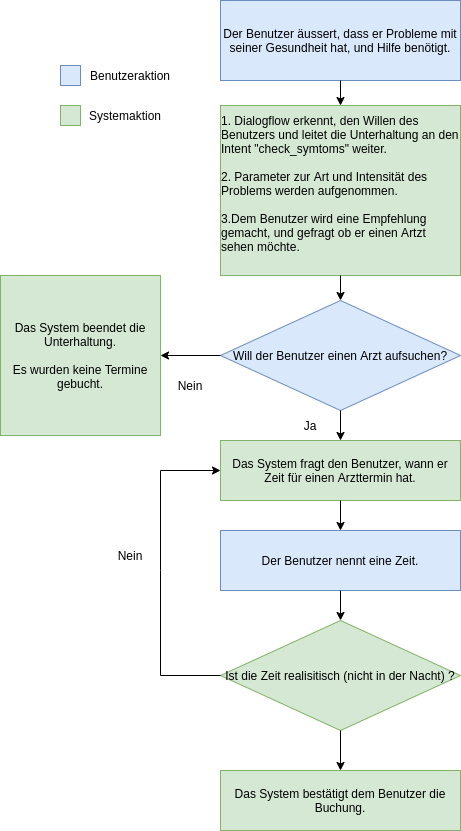
\includegraphics[width=0.6\linewidth]{backendOverview.png}
                \caption{Backend Übersicht-Flowchart}
                \label{fig:backEndFlowChart}
            \end{center}
        \end{figure}
        \newpage

    \subsection{Intents}
        \paragraph{}
            Das Backend ist in 4 Intents strukturiert
            \begin{figure}[h!]
                \begin{center}
                    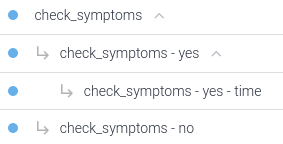
\includegraphics[width=0.5\linewidth]{intents.png}
                    \caption{Dialogflow intent liste}
                    \label{fig:intentslist}
                \end{center}
            \end{figure}
    \subsection{Aufnahme von Symptomen}
        \paragraph{}
            Im ersten Intent, des Dialogs - "check\_symtpoms" - wird eine Liste an
            symptomen, sowie ein Schmerzniveau und die Zeitdauer, seit dem die Symptome
            bestehen, aufgenommen.

        \paragraph{}
            Folgende Trainingssätze, wurden für das Auslösen des Intents definiert:
            \begin{itemize}
                \item i have \emph{pain} since \emph{yesterday}
                \item i have \emph{pain}
                \item i need help
                \item should i go to the doctor?
                \item Can you tell me if i should seee a doctor?
                \item Am I sick?
                \item I feel Sick
                \item feel \emph{unwell}
            \end{itemize}
            Wobei, hier \emph{kursiv} geschrieben Wörter auf entsprechende Parameter gematcht wurden.

        \subsubsection{Parameter Entities}
            Um die Symptom-Parameter aufzuzeichnen wurden folgende Parameter und Entities definiert:
            \begin{table}[!h]
                \begin{center}
                    \begin{tabular}{c|c}
                        \textbf{Parameter} & \textbf{Entity}\\
                        \hline
                        SymType & symptom\_type\\
                        SymIntensity & symtom\_intensity\\
                        SymDuration & System.Date
                    \end{tabular}
                    \caption{Paramter und Entities}
                    \label{tab:tabelleParamsUndEntities}
                \end{center}
            \end{table}
            
            \paragraph{}
                \textbf{symtom\_type} hat einen Wertebereich von: pain, unwell,
                sick, fever, cough, loss of taste, chestpain, tiredness und shortness of breath. Mit jeweils 3 bis 4 
                Synonymoen.
            
            \paragraph{}
                \textbf{symtom\_intensity} hat einen Wertebereich von 1 bis 5 jeweils Wörtltlich (z.B. "One", "Eins") und
                Buchstäblich (z.B. 1).
            
            \paragraph{}
                \textbf{System.Date} ist ein vorgefertigtes Entity mit einem Wertebereich, welcher beliebige Kalenderdaten
                enthalten kann.
    \subsection{Auswertung der Symptome}
        \paragraph{}
            In einem zweiten Schritt geht es nun darum die Angaben auszuwerten, damit dem Patienten tipps, zu weiterem verhalten
            gegeben werden können. Die Auswertung findet am ende des Intents statt, indem ein Webhook aufgerufen wird.
            Hier ist als Antwort auf den entsprechenden Intent "check\_symptoms" eine entsprechende Funktion "checkSymptoms" (Siehe: Abbildung \ref{fig:checksymptomsfunction})
            registriert.
        \begin{figure}[h!]
            \begin{center}
                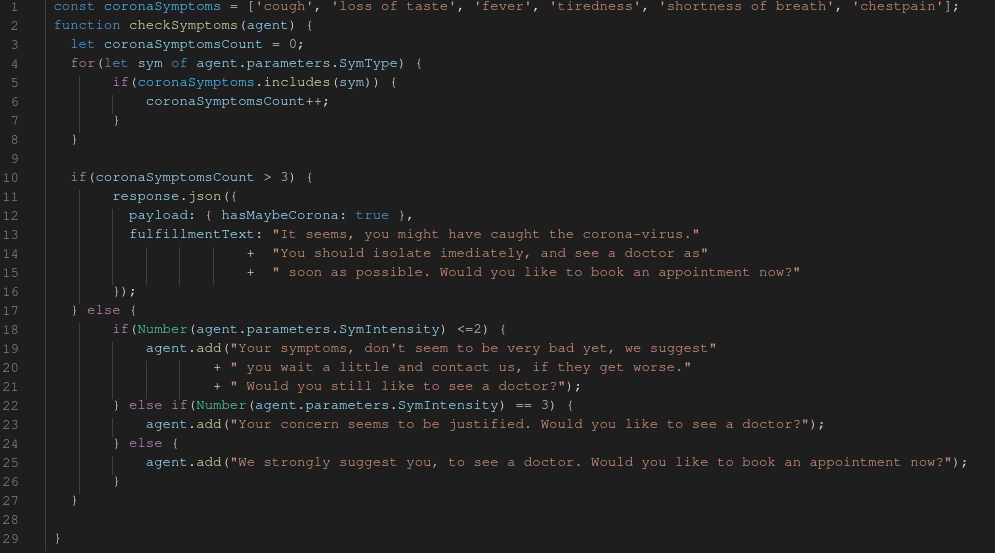
\includegraphics[width=\linewidth]{checkSymptoms.png}
                \caption{checkSymptoms Funktion}
	            \label{fig:checksymptomsfunction}
            \end{center}
        \end{figure}
        \paragraph{}
            Auf den Zeilen 3 bis 8 werden die angegebenen Symptome mit dem Array \emph{coronaSymptoms} verglichen und gezählt.
            Auf Zeile 10 wird überprüft, ob die Anzahl der auf Corona-Symptome passenden Symptome grösser als 3 Ist. Ist dies
            der Fall wird unabhängig der anderen Parameter eine Entsprechende Nachricht zurückgesandt, welche den Benutzer über
            diesen Umstand informiert, und ihm vorschlägt, sich zu isolieren und testen zu lassen.

        \paragraph{}
            Besteht kein verdacht auf das Corona-Virus, so ist die Symtomstärke ("symtom\_intensity") Ausschlaggebend für die Antwort:
            \begin{itemize}
                \item Intensität kleiner oder gleich 2: Die Symptome scheinen nicht schlimm zu sein. Dem Benutzer wird geraten abzuwarten und bei
                    verschlimmerung des zustands einen Arzt aufzusuchen. Der Benutzer wird gefragt ob er dennoch einen Arzttermin buchen
                    möchte
                \item Intensität = 3: Der Benutzer wird gefragt, ob er einen Arzttermin buchen möchte.
                \item Intensität grösser 3: Dem Benutzer wird angeraten einen Arzt aufzusuchen. Er wird gefragt, ob er einen entsprechenden Termin
                    buchen möchte.
            \end{itemize}

        \paragraph{}
            Alle Antworten, fragen den Benutzer, ob er einen Arzttermin buchen will. Mit den Intents \emph{check\_symptoms - yes} und \emph{check\_symptoms - no}
            (Siehe: Abbildung \ref{fig:intentslist}) wird die Antwort des Benutzers abgefangen. Während \emph{check\_symptoms - no} zu einer Verabschiedungsantwort führt,
            fragt \emph{check\_symptoms - yes} direkt, danach wann der Termin stattfinden soll.

    \subsection{Termin buchen}
        \paragraph{}
            Der Intent \emph{check\_symptoms - yes - time} fängt die Antwort des vorgehenden Intents (Frage nach Terminzeit) direkt ab und löst im Webhook
            eine weitere Methode aus (Abbildung \ref{fig:handleappointmentfunction}).
        \begin{figure}[h!]
            \begin{center}
                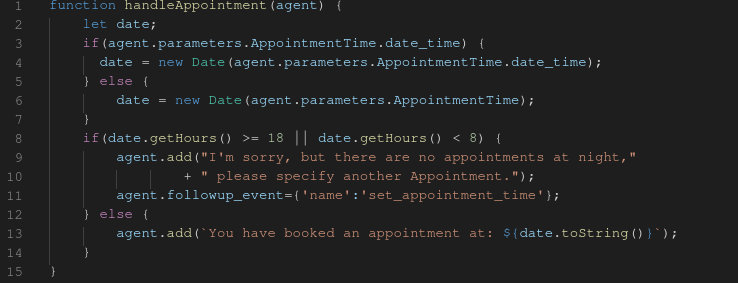
\includegraphics[width=0.7\linewidth]{handleAppointmentFunction.png}
				\caption{handleAppointment Funktion}
	            \label{fig:handleappointmentfunction}
            \end{center}
        \end{figure}

        \paragraph{}
            Die ersten 7 Zeilen der Funktion kümmern sich um das Parsen des Datums. Da dieses nicht immer gleich daher kommt,
            musste ein wenig logik, zur überprüfung der Daten implementiert werden. Zeile 8 prüft, ob die Uhrzeit zwischen 08:00
            und 20:00 Uhr liegt. Alles zwischen diesen zwei Zeitpunkten ist als gültige Uhrzeit definiert, und führt dazu, dass die
            Buchung auf Zeile 13 bestätigt wird. Der Dialog ist hiermit beendet. Liegt die Zeit allerdings ausserhalb des gültigen
            Bereichs, wird auf den Zeilen 9 und 10 eine Fehlernachricht zurückgegeben und nach einer neuen Zeit gefragt.
            Auf Zeile 11 wird als Folgeintent das Event \emph{set\_appointment\_time} definiert. Dieses Event zeigt auf denselben 
            Intent, auf dem wir gerade operieren (\emph{check\_symptoms - yes - time}). Die Terminbuchung wird also wiederholt, bis
            eine gültige Zeit für den Termin angegeben wird. 

        \begin{figure}[h!]
            \begin{center}
                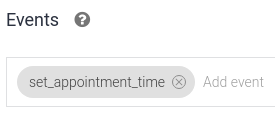
\includegraphics[width=0.5\linewidth]{eventSetting.png}
				\caption{Eventeinstellung für die Schleifenlogik}
            	\label{fig:eventSetting}
            \end{center}
        \end{figure}
 
\newpage

\section{Discussion}
    \subsection{Was wir gelernt haben}
        \paragraph{}
            Bei der Umsetzung dieses Projekts, haben wir gelernt, dass die Dialogflow Plattform sich äusserst gut eignet, um Schnittstellen
            zwischen Menschen und Informatiksystemen zu konstruieren. Die so erschaffenen Benutzeroberflächen sind, wenn richtig umgesetzt,
            sehr intuitiv zu bedienen. Sehr viel potential bietet diese Technologie aus unserer sicht auch, wenn es darum geht, Menschen mit
            körperlichen Einschrännkungen, den zugang zu diversen Programmen zu verschaffen. Das bekannteste Beispiel sind dabei moderne Sprachassistenten.
    \subsection{Limitationen}
        \paragraph{}
            Wenn man an AI denkt, geht man schnell davon aus, dass sich eine Interaktion mit einem System kaum noch von einer Interaktion mit einem
            Menschen unterscheidet. Dies mag vielleicht in Zukunft der Fall sein, ist es aber heute noch nicht. 
        \paragraph{}
            Dialogflow, kommt schnell an seine Grenzen, wenn man den Chat-Bot mit ungenauen oder zusätzlichen (unnötigen) Informationen beliefert,
            für die er nicht trainiert wurde. 
    \subsection{Erweiterungsmöglichkeiten unserer Arbeit}
        \paragraph{}
            Um die Aufnahme der Informationen weiter zu verbessern, könnte der Satz an Trainingssätzen erweitert werden, sodass es weniger häufig
            zu Misverständinissen, durch einfache Schreibfehler kommt.
        \paragraph{}
            Weiter könnte man unseren Chatbot durch folgende features erweitern um ihn für einen produktiven Einsatz vorzubereiten:
            \begin{itemize}
                \item Buchungssystem mit persistenten Daten und konfliktauflösung.
                \item Zuweisung von Patienten an Ärzte mit unterschiedlichen Spezialisierungen, anhand der Symptome.
                \item Implementation eines Webinterfaces oder Interface mit einem Sprachassistenten. 
            \end{itemize}

\end{document} 
